\documentclass[tikz]{standalone}

\usetikzlibrary{calc}

\begin{document}
	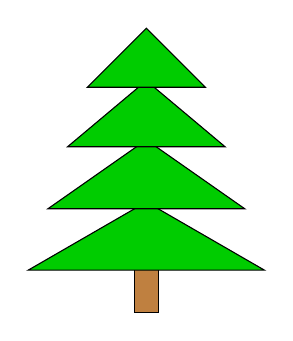
\begin{tikzpicture}
		\pgfmathsetmacro{\trunkwidth}{0.3}
		\pgfmathsetmacro{\trunkheight}{0.6}
		\pgfmathsetmacro{\crownbaseangle}{30}
		\pgfmathsetmacro{\crownangleincrease}{5}
		\pgfmathsetmacro{\crownbasewidth}{3}
		\pgfmathsetmacro{\crownwidthdecrease}{0.5}
		\pgfmathsetmacro{\cutout}{0.9}
		
		\draw[fill=brown] (-\trunkwidth/2,0) rectangle +(\trunkwidth, \trunkheight);
		\coordinate (height0) at (0, \cutout * \trunkheight);
		\foreach \i[count=\j] in {0, 1, ..., 3}
		{
			\pgfmathsetmacro{\baselength}{\crownbasewidth - \i * \crownwidthdecrease}
			\pgfmathsetmacro{\smallangle}{\crownbaseangle + \i * \crownangleincrease}
			\pgfmathsetmacro{\largeangle}{180 - 2 * \smallangle}
			\pgfmathsetmacro{\sidelength}{0.5 * \baselength / cos(\smallangle)}
			\draw[fill=green!80!black] 
				(height\i) -- 
				++(\baselength / 2, 0) -- 
				++({180-\smallangle}:\sidelength) coordinate (here\i) --
				++({360-\smallangle-\largeangle}:\sidelength) --
				cycle;				
			\coordinate (height\j) at ($(height\i)!\cutout !(here\i)$);
		}
	\end{tikzpicture}
\end{document}
